\documentclass[pdflatex,sn-mathphys-num]{sn-jnl}

\usepackage{graphicx}
\usepackage{amsmath,amssymb,amsfonts}
\usepackage{xcolor}
\usepackage{textcomp}
\usepackage{booktabs}

\setlength{\textfloatsep}{6pt plus 2pt minus 4pt}
\setlength{\floatsep}{4pt plus 2pt minus 2pt}
\setlength{\intextsep}{4pt plus 2pt minus 2pt}
\setlength{\abovecaptionskip}{4pt}
\setlength{\belowcaptionskip}{2pt}
\renewcommand{\arraystretch}{0.88}

\raggedbottom

\begin{document}

\title[Livestock Sector Forecasting in Kenya]{Livestock Sector Forecasting in Kenya: A Cohort-Based Quarterly Analysis on Population, Production, and Feed Demand}

\author*[1]{\fnm{Natasha} \sur{Wavomba}}% ORCID: 0000-0000-0000-0000
\author[1]{\fnm{Maria} \sur{Ogamba}}% ORCID: 0009-0006-5814-4009
\author[1]{\fnm{Lorraine} \sur{Eyinda}}% ORCID: 0000-0000-0000-0000
\author[1]{\fnm{Joseph} \sur{Gitonga}}% ORCID: 0000-0002-0607-2828
\author[1]{\fnm{John} \sur{Olukuru}}% ORCID: 0000-0002-8534-2346
\author[1]{\fnm{Joseph} \sur{Sevilla}}% ORCID: 0000-0002-9112-824X

\affil*[1]{\orgdiv{@iLabAfrica}, \orgname{Strathmore University}, \orgaddress{\city{Nairobi}, \country{Kenya}}}

\abstract{% Abstract

Kenya's livestock sector contributes 42\% of agricultural GDP and 12\% of national GDP, yet quantitative planning remains constrained by the absence of reproducible, data-driven analytical models. This study presents a cohort-based quarterly forecasting framework spanning nine value chains: dairy cattle, beef cattle, camels, goats, sheep, poultry, pigs, rabbits, and apiculture, initialized from the 2019 KNBS livestock census with projections from 2020 to 2041. The model applies a quarterly transition sequence covering mortality, culling, offtake, age-based maturation, and reproduction across all cohorts. Production modules translate herd and flock dynamics into species-specific output metrics, while a feed demand module estimates dry matter requirements by species and agro-ecological zone. Projected outputs indicate a CAGR of 3.6-6\% across all value chains. Beyond forecasting, the framework exposes productivity bottlenecks and structural inefficiencies, including feed deficits, low offtake rates, and suboptimal reproductive performance, that aggregate assessments typically obscure. The model provides an analytical basis for food security planning, targeted infrastructure investment, and evidence-based livestock policy.}

\keywords{Livestock model forecasting, cohort population model, biological parameters}

\maketitle

\section{Introduction}

In most African countries, the livestock sector supports the livelihoods of millions of rural households and plays an important role in poverty reduction. In livestock-rich countries such as Kenya, the sector contributes substantially to the national economy while providing income, employment, and food security across both rural and urban populations. Beyond primary production, livestock also supports employment throughout value chains, including dairy, meat, and leather processing industries. The livestock sector plays a major role in Kenya's food system, contributing approximately 12\% of the country's Gross Domestic Product (GDP), 40\% of agricultural GDP, and 22\% of the food system GDP \cite{bahtaLivestockSectorTransformation2023}.

Kenya's population is projected to reach approximately 96 million by 2050, with nearly half of the population residing in urban areas. Consequently, demand for animal-source foods is expected to increase substantially owing to population growth, urbanization, rising incomes, and changing dietary preferences \cite{bahtaLivestockSectorTransformation2023}. Meeting this growing demand will require sustained improvements in livestock productivity, efficient management of feed and water resources, and evidence-based planning to support the sustainable development of the livestock sector. Reliable forecasting frameworks that project livestock populations, production outputs, feed demand, and resource requirements are therefore essential for evidence-based planning, strategic investment, and sustainable livestock sector development.

Statistical time-series models are commonly used to forecast livestock populations using historical data. These methods estimate future livestock numbers based on past population trends and have been applied to support livestock planning and management. \cite{bahtaLivestockSectorTransformation2023} used autoregressive and probabilistic time-series models to forecast pig populations, while Ozbek compared autoregressive integrated moving average (ARIMA) and artificial neural network (ANN) models for forecasting cattle populations in Türkiye. Similarly, \cite{bahtaLivestockSectorTransformation2023} applied exponential smoothing to forecast beef cattle populations in Indonesia. Although these methods have demonstrated good predictive performance, they rely primarily on historical trends and do not explicitly represent biological processes such as reproduction, mortality, maturation, culling, and offtake. Consequently, their ability to evaluate the effects of biological parameters and management interventions on future livestock population dynamics is limited.

In contrast to statistical forecasting approaches, biological simulation models explicitly represent the demographic processes governing livestock populations. Animals are grouped into cohorts according to age, sex, or production stage, with transitions driven by biological processes such as reproduction, maturation, mortality, culling, and replacement. These models offer a biologically realistic representation of herd dynamics and enable the evaluation of alternative management strategies. \cite{bahtaLivestockSectorTransformation2023} developed an age- and sex-structured cattle population model that incorporates management practices and animal movements to simulate herd dynamics. Such models serve as valuable decision-support tools by linking biological processes to herd structure and productivity, they are generally developed for specific livestock species or production systems and do not explicitly integrate livestock population dynamics, production, environmental carrying capacity, and feed demand within a unified forecasting framework. Consequently, there remains a lack of reproducible analytical frameworks that simultaneously integrate livestock population dynamics, production, environmental carrying capacity, and feed demand to support long-term livestock sector planning.

To address these limitations, this study develops a cohort-based quarterly forecasting framework for Kenya's nine principal livestock value chains. The framework explicitly models biological cohort transitions through reproduction, mortality, maturation, culling, and offtake while linking livestock population dynamics to species-specific production, environmental carrying capacity, and feed demand across agro-ecological zones. By integrating these components within a single modelling framework, the proposed approach provides a comprehensive decision-support tool for forecasting livestock populations, production, and resource requirements, thereby supporting evidence-based livestock planning and policy development in Kenya.


\section{Literature Review}

\subsection{Significance of the Livestock Sector in Kenya}

Livestock production plays an important role in Kenya's economy and household livelihoods through income generation, employment, wealth accumulation and food provision. At the farm level, livestock generates income through the sale of livestock-derived foods and other products such as hides and skins, while livestock ownership also serves as a form of savings and wealth accumulation, particularly in pastoral communities % TODO: cite (Ayan et al., 2020; Baltenweck et al., 2020) 

Approximately 80\% of Kenya’s land is arid to semi-arid lands (ASALs) mainly used for extensive pastoralism. The ASALs are estimated to support about 25\% of the nation’s human population and just over 50\% of its livestock and the livestock sector accounts for 90\% of employment and over 95\% of household income. It contributes significantly to the economy of Kenya with livestock production accounting to 50\% of agricultural GDP which in turn is 20 - 30\% of total GDP % TODO: cite (Kabubo-Mariara, 2009; Nyariki & Amwata, 2019) 

According to projections from the Kenya National Bureau of Statistics (KNBS), the country’s population will continue to grow and may reach about 96 million by 2050 with almost 50\% living in urban areas % TODO: cite (FAO 2019; Macmillan 2019). Along with this pop growth, demand for animal-source foods is expected to grow substantially, as more affluent and more urban consumers demand nutrient-rich foods and more diversified diets % TODO: cite (FAO 2019). This change in demand may lead to exponential growth in the livestock sector creating new business opportunities along the livestock value chains.

\subsection{Historical trends in livestock population and production }

Historical trends in Kenya's livestock population and production provide an important basis for understanding the evolution of the livestock sector and its future dynamics. Evidence from different periods indicates that livestock populations have followed different trajectories across species and over time % TODO: cite (FAO, 2002). Production trends also reflect such heterogeneity. Beef, mutton and goat meat, pig meat, poultry meat, eggs and milk had different production trajectories between 2010 and 2019 % TODO: cite (FAOSTAT, 2022). This variation suggests that livestock commodities are not necessarily responding to the same production dynamics and thus provides an argument for considering livestock biological assumptions in the investigation of future population and production trends. 

\begin{figure}[htbp]
    \centering
    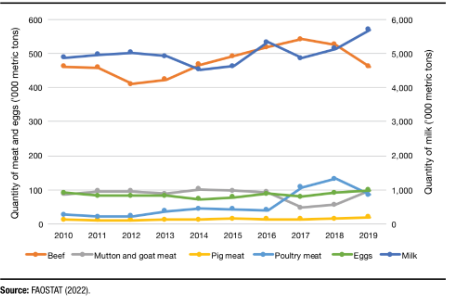
\includegraphics[width=0.9\textwidth]{figures/FAOSTAT_production_trends.png}
    \caption{Trends in selected livestock production in Kenya, 2010--2019.}
    \label{fig:livestock-production-trends}
    \caption*{\textit{Source: FAOSTAT (2022).}}
\end{figure}

Historical trends of livestock production also suggest a close association between changes in output and changes in livestock numbers, but not necessarily in proportional terms. At continental level, the African Union’s Livestock Development Strategy for Africa states that increases in herd and flock size have contributed significantly to the growth in the supply of beef, milk, poultry and sheep and goat meat % TODO: cite (African Union, 2015). This finding suggests that population dynamics should be understood in the future assessment of livestock supply and that the growth of livestock populations may add to total production without being reflected in equivalent productivity increases. 

Evidence from Kenya’s smallholder dairy sector further illustrates the relationship between livestock population structure and production. % TODO: cite Wanjala and Njehia, (2014) noted that poor performance of dairy herd was associated with inadequate replacement stock, limited access to improved breeding animals, inadequate feed quantity and quality, breed characteristics and short lactation periods. The results are dairy cattle specific, but they do suggest a substantial consideration for livestock population and production analysis in general. 

Taken together, the historical evidence suggests that the evolution of livestock populations and the productive characteristics of those populations should both be taken into account in forecasting livestock production. The variation across livestock commodities and the importance of herd structure and replacement dynamics identified in previous studies also imply that forecasts based purely on aggregate historic growth rates may overlook changes that occur within livestock populations over time. A more disaggregated approach can therefore be a basis for studying how changes in livestock numbers translate into production and then into livestock feed requirements. This allows for cohort-based forecasts of livestock population, production and feed demand for Kenya’s livestock value chains.

\subsection{Modelling Approaches for Livestock Population and Production Forecasting}

Different modeling approaches have been used in past studies to project future livestock production and supply. A common approach is extrapolation of historical growth rates in which past trends in production are used to generate probabilistic estimates of future livestock supply. Other studies have used exploratory scenario-based models which start from current production conditions and assess how different drivers, trends and interactions may influence future livestock production  % TODO: cite (Wiebe et al., 2018). 

More sophisticated approaches integrate economic relationships with biophysical factors such as land-system changes, crop physiology and water availability to estimate future agricultural and livestock supply, including integrated assessment and partial-equilibrium models  % TODO: cite (Robinson et al., 2015). Projections have also been developed in Kenya based on assumptions of changes in livestock production over time. 

Statistical modeling approaches have also been used to explore factors that drive livestock productivity in Kenya. For instance,  % TODO: cite Ajak et al. (2020) employed linear regression to assess the relationship between productivity of dairy cattle and factors including concentrate feeding, breed and disease. The analysis found a positive association between milk production and concentrate feeding in early lactation, and reproductive and productive performance was associated with management and production-related factors. The primary aim of such regression-based approaches, however, is explanatory rather than predictive. However regression models can provide an important basis for forecasting by identifying production drivers that may be incorporated as explanatory variables in future livestock production models. 

\subsection{Cohort-Based Herd Dynamics, Population and Production Projection Models}

Cohort-based, age and sex-stratified models divide livestock populations into biologically meaningful groups and simulate movement through successive stages based on reproduction, maturation, mortality and removal rates. An early basis for this approach was the ILCA cattle herd-dynamics model of % TODO: cite Konandreas and Anderson (1982). The model simulated herd development in a stochastic demographic framework for evaluating production alternatives. Later stage-structured approaches, e.g. % TODO: cite  Hary (2004), showed that sustainability of livestock production depends not only on herd size but also on the demographic composition of the herd and on the pattern of animal off-take. 

Empirical applications have highlighted the significance of explicitly considering the population structure of livestock. For example, % TODO: cite  Lesnoff, Corniaux and Hiernaux (2012) used a demographic model to study the recovery of the cattle population after drought and showed that the recovery was particularly sensitive to reproductive performance. Likewise, % TODO: cite  Tuffa and Treydte (2017) developed a stochastic age and sex-structured model for Boran cattle which included demographic processes, carrying capacity, market conditions and herder decisions. Their results suggested that decisions to remove animals from different demographic groups can drastically change population trajectories. Combined, these studies indicate that livestock population projections are more informative when they include the demographic processes by which populations are replenished, mature and removed, rather than just using aggregate growth rates. 

\subsection{Biological Transition Parameters: Mortality, Reproduction, Maturation and Off-take}

Studies from across Sub-Saharan Africa have documented significant differences in mortality, fertility, maturation and off-take rates across livestock species and production environments. In a systematic review of livestock production parameters, % TODO: cite Otte and Chilonda (2002) summarized the relative high mortality of young cattle and small ruminants, low reproductive performance and generally low off-take in traditional production systems. Their synthesis also showed that population growth rates vary widely among species and production systems, emphasizing the necessity of biologically and geographically relevant transition parameters. Off-take is important especially as animals may leave the herd by sale or slaughter before the end of their biological life. These processes imply that the observed changes in livestock population are the net result of births, maturation, mortality and removals. 

\subsection{Production-System Modelling Across Livestock Value Chains}

Population projections need to be converted into production with parameters reflecting the biological and management characteristics of individual livestock value chains. As earlier research in Kenya has shown, there are large variations in productivity between livestock species and production systems. For example, research on smallholder dairy systems has found relatively low milk yields, long calving intervals and large feed-related productivity constraints % TODO: cite (Kashongwe et al., 2017). Studies of genetics have also revealed that patterns of lactation in smallholder systems differ from those under intensive production conditions, adding to the need for production parameters that are indicative of the local production environments % TODO: cite (Ojango et al., 2019). 

A similar differentiation is needed in other value chains. For instance, the Kenyan poultry sector is characterized by distinct indigenous and commercial production systems with very different population dynamics and production characteristics % TODO: cite (Magothe et al., 2012). Population changes are also converted into meat output in beef and small ruminant systems thru species and system specific growth and offtake characteristics. Camel production is a growing component of livestock-based livelihoods in the arid and semi-arid lands. International frameworks such as FAO's GLEAM also connect livestock populations with species-specific production outputs % TODO: cite (FAO, 2018). The studies suggest that a single population to production relationship may not adequately capture the diversity of the Kenyan livestock sector, thereby justifying the use of production parameters that are specific to each value chain. 

\subsection{Carrying Capacity, Feed Availability and Feed Demand}

Availability of feed resources also limits the growth of the livestock population. Studies of carrying capacity in African rangelands show that livestock numbers must be matched against available forage, and remote-sensing studies have increasingly made it possible to include seasonal and spatial variation in forage availability in livestock assessments % TODO: cite (Meshesha et al., 2019). 

Conventional livestock feed balance methods calculate how dry matter animals need by looking at their body weight or using livestock unit equivalents. Common intake rates like the 2.5 percent of body weight per day standard have been helpful for figuring out how much feed animals need when doing livestock assessments % TODO: cite (Rivière, 1991; Kearl, 1982). Applications across Sub-Saharan Africa have used these approaches to identify substantial and often seasonal feed deficits. These developments suggest that livestock population and production projections can provide a useful basis for estimating future feed requirements. 

\subsection{Research Gap}

The reviewed literature establishes each component of the present study on solid empirical and methodological ground: cohort-structured herd models are validated and generalisable % TODO: cite (Konandreas & Anderson, 1982; Hary, 2004; Lesnoff et al., 2012; Tuffa & Treydte, 2017); biological transition parameters for Sub-Saharan systems are documented in synthesis form % TODO: cite (de Leeuw & Wilson, 1988; Otte & Chilonda, 2002); species-specific production has been characterised across Kenya's key value chains % TODO: cite (Magothe et al., 2012; Kashongwe et al., 2017; Ojango et al., 2019); satellite-based forage and carrying-capacity estimation researched % TODO: cite (Meshesha et al., 2019); dry-matter feed-balance methods are standardised % TODO: cite (Rivière, 1991; Kearl, 1982); and integrated scenario frameworks have demonstrated policy relevance for Kenya % TODO: cite (Bosire et al., 2022; FAO, 2018).

What remains scarce is a single, reproducible, biologically grounded framework that unifies these strands for Kenya. One that simultaneously (i) spans all nine key value chains rather than a single species, (ii) advances cohort transitions at a quarterly time step to capture seasonality, (iii) endogenously constrains herd growth through a dynamic feed-supply balance driven by satellite-derived carrying capacity, and (iv) closes the loop from population to species-specific production to disaggregated feed demand. Existing Kenyan analyses are typically either static inventories % TODO: cite (KNBS, 2019), single-value-chain studies, or top-down economic-scenario projections that do not resolve underlying herd demography. By integrating these elements into one coherent, parameter-transparent architecture, the present study addresses a clear and consequential gap, offering not only defensible forecasts but a diagnostic instrument for identifying the feed deficiencies, low off-take rates and reproductive bottlenecks that aggregate assessments obscure.


\input{sections/03_methodology}
% ---------------------------------------------------------------
% Results section. Preamble requirements:
%   \usepackage{booktabs}
%   \usepackage{graphicx}
% For Calibri body text, compile with XeLaTeX or LuaLaTeX and add:
%   \usepackage{fontspec}
%   \setmainfont{Calibri}          % or \setmainfont{Carlito} on Linux
% (The figures are already set in Calibri/Carlito.)
% Figures expected in the same directory as this file:
%   ruminant_pop.png  ruminant_prod.png  ruminant_feed.png
%   nonrum_pop.png    nonrum_prod.png    nonrum_feed.png
% ---------------------------------------------------------------

\section{Results and Discussion}

Population and production are reported over 2019--2041. The 2019 values are
historical observations; 2020--2041 are model projections. The 2019 baseline is
therefore shown shaded in the figures, with the 2019--2020 segment drawn dotted,
and where the transition from historical to projected data produces a step
(Section~\ref{sec:dq}) growth rates are quoted from 2020. Feed demand carries no 2019
historical value and is reported over 2020--2041 throughout. 

\subsection{Population}

\subsubsection{Ruminants}

Total ruminant numbers rise from 88.0 million head in 2019 to 272.1 million in
2041, a 3.1-fold increase equivalent to 5.3\,\% per year (Table~\ref{tab:rumpop},
Figure~\ref{fig:rumpop}). Growth is not evenly distributed across value chains. Beef cattle expand
fastest at 6.6\,\% per year, quadrupling to 67.8 million head and overtaking
sheep as the second-largest ruminant population in 2036. Goats remain the
largest single population throughout, growing 5.9\,\% per year to 121.3 million.
Camels and dairy cattle follow intermediate trajectories of 5.2\,\% and
4.9\,\% per year respectively, each roughly tripling. Sheep are the
slowest-growing ruminant chain at 3.3\,\% per year, doubling over the period;
their share of the ruminant herd falls from 31.2\,\% in 2019 to
20.5\,\% in 2041.

\begin{table}[htbp]
\centering
\caption{Ruminant population, 2019--2041 (thousand head)}
\label{tab:rumpop}
\small
\begin{tabular}{lrrrrrr}
\toprule
\textbf{Series} (\,000 head) & \textbf{2019} & \textbf{2025} & \textbf{2030} & \textbf{2035} & \textbf{2041} & \textbf{CAGR 2019--41 (\%)} \\
\midrule
Goats & 34\,658 & 50\,854 & 66\,733 & 87\,571 & 121\,333 & 5.9 \\
Beef cattle & 16\,640 & 23\,168 & 32\,365 & 45\,282 & 67\,767 & 6.6 \\
Sheep & 27\,441 & 33\,099 & 39\,221 & 46\,098 & 55\,665 & 3.3 \\
Camels & 4\,722 & 6\,661 & 8\,535 & 10\,794 & 14\,265 & 5.2 \\
Dairy cattle & 4\,537 & 5\,929 & 7\,593 & 9\,726 & 13\,091 & 4.9 \\
\textbf{Total ruminants} & 87\,998 & 119\,710 & 154\,448 & 199\,470 & 272\,119 & 5.3 \\
\bottomrule
\end{tabular}
\end{table}

\begin{figure}[htbp]
\centering
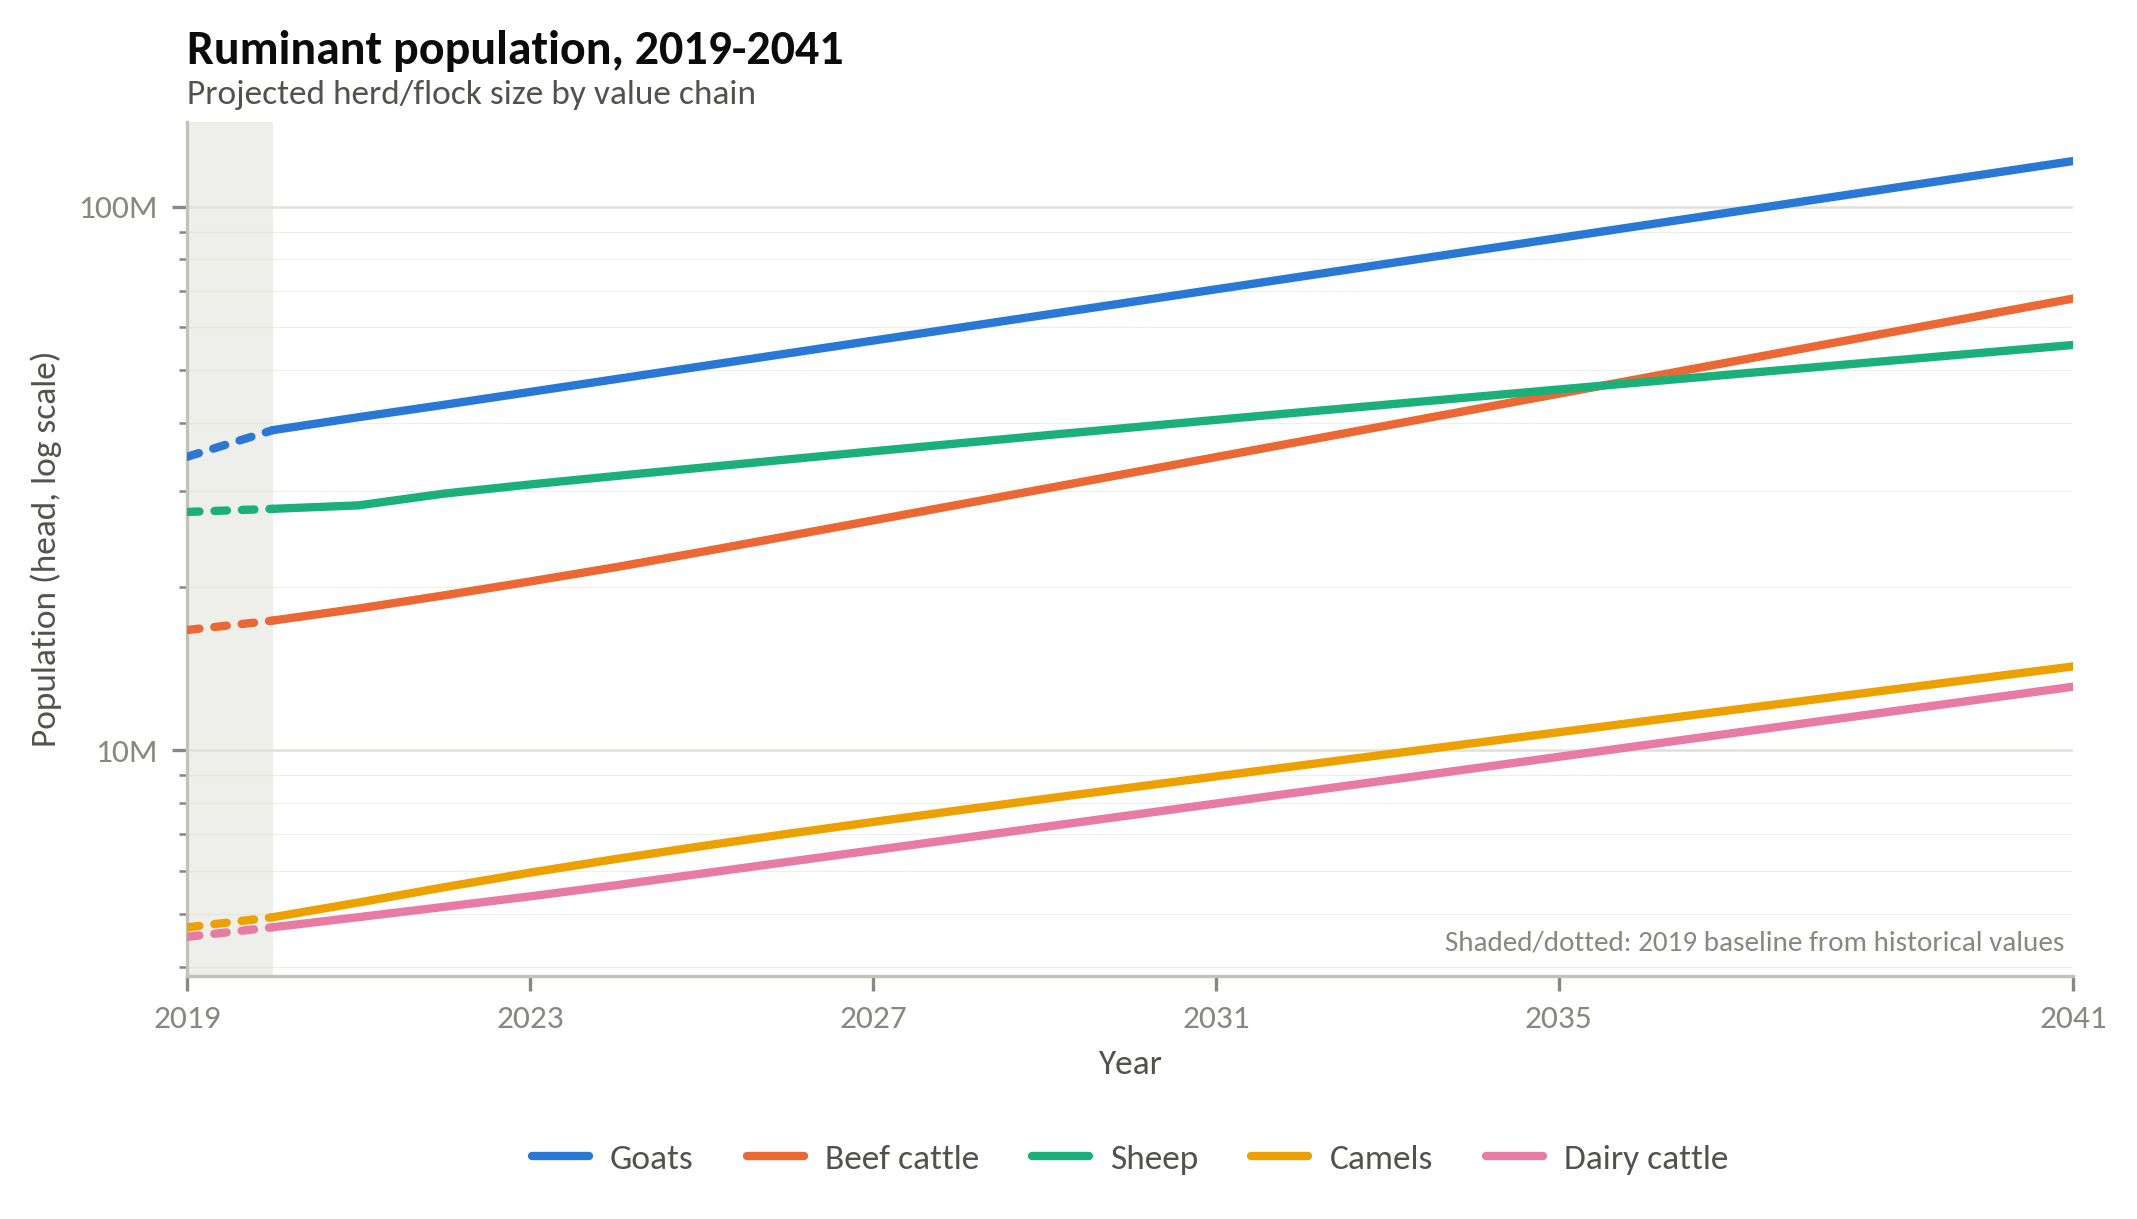
\includegraphics[width=\textwidth]{ruminant_pop.png}
\caption{Projected ruminant population by value chain, 2019--2041. Logarithmic vertical axis; the shaded band and dotted segment mark the 2019 baseline, which is a historical value.}
\label{fig:rumpop}
\end{figure}

\subsubsection{Non-ruminants}

Non-ruminant numbers grow far more slowly, from 106.3 million head in 2019 to
159.1 million in 2041, a 1.5-fold increase at 1.8\,\% per year
(Table~\ref{tab:nrpop}, Figure~\ref{fig:nrpop}). The aggregate conceals a divergence between the commercial and non-commercial segments of the poultry
chain. Layers and broilers expand by only about
10\,\% over 22 years (0.4\,\% per year) and plateauing after the early 2030s,
whereas indigenous poultry grow steadily at 3.0\,\% per year to 89.3 million
birds. The composition of the poultry flock shifts accordingly: indigenous birds
rise from 44.1\,\% to 58.1\,\% of total poultry, while the combined layer and
broiler share of all non-ruminants falls from 55.2\,\% to 40.5\,\%. The smallest
chains grow fastest: rabbits 4.4-fold at 7.0\,\% per year and pigs 3.5-fold at
5.9\,\% per year. Both start below one million head, so they remain marginal in
absolute terms. Managed bee colonies increase 2.7-fold to 3.5 million.

\begin{table}[htbp]
\centering
\caption{Non-ruminant population, 2019--2041 (thousands). Bee colonies are reported separately and excluded from the total.}
\label{tab:nrpop}
\small
\begin{tabular}{lrrrrrr}
\toprule
\textbf{Series} (\,000) & \textbf{2019} & \textbf{2025} & \textbf{2030} & \textbf{2035} & \textbf{2041} & \textbf{CAGR 2019--41 (\%)} \\
\midrule
Indigenous poultry & 46\,293 & 54\,774 & 65\,960 & 75\,970 & 89\,288 & 3.0 \\
Broilers & 45\,838 & 47\,477 & 49\,975 & 50\,175 & 50\,386 & 0.4 \\
Layers & 12\,844 & 13\,114 & 13\,946 & 14\,030 & 14\,089 & 0.4 \\
Rabbits & 737 & 1\,149 & 1\,585 & 2\,191 & 3\,235 & 7.0 \\
Pigs & 596 & 817 & 1\,097 & 1\,471 & 2\,088 & 5.9 \\
\textbf{Total (excl.\ colonies)} & 106\,309 & 117\,331 & 132\,563 & 143\,837 & 159\,086 & 1.8 \\
Bee colonies & 1\,289 & 1\,838 & 2\,384 & 2\,926 & 3\,489 & 4.6 \\
\bottomrule
\end{tabular}
\end{table}

\begin{figure}[htbp]
\centering
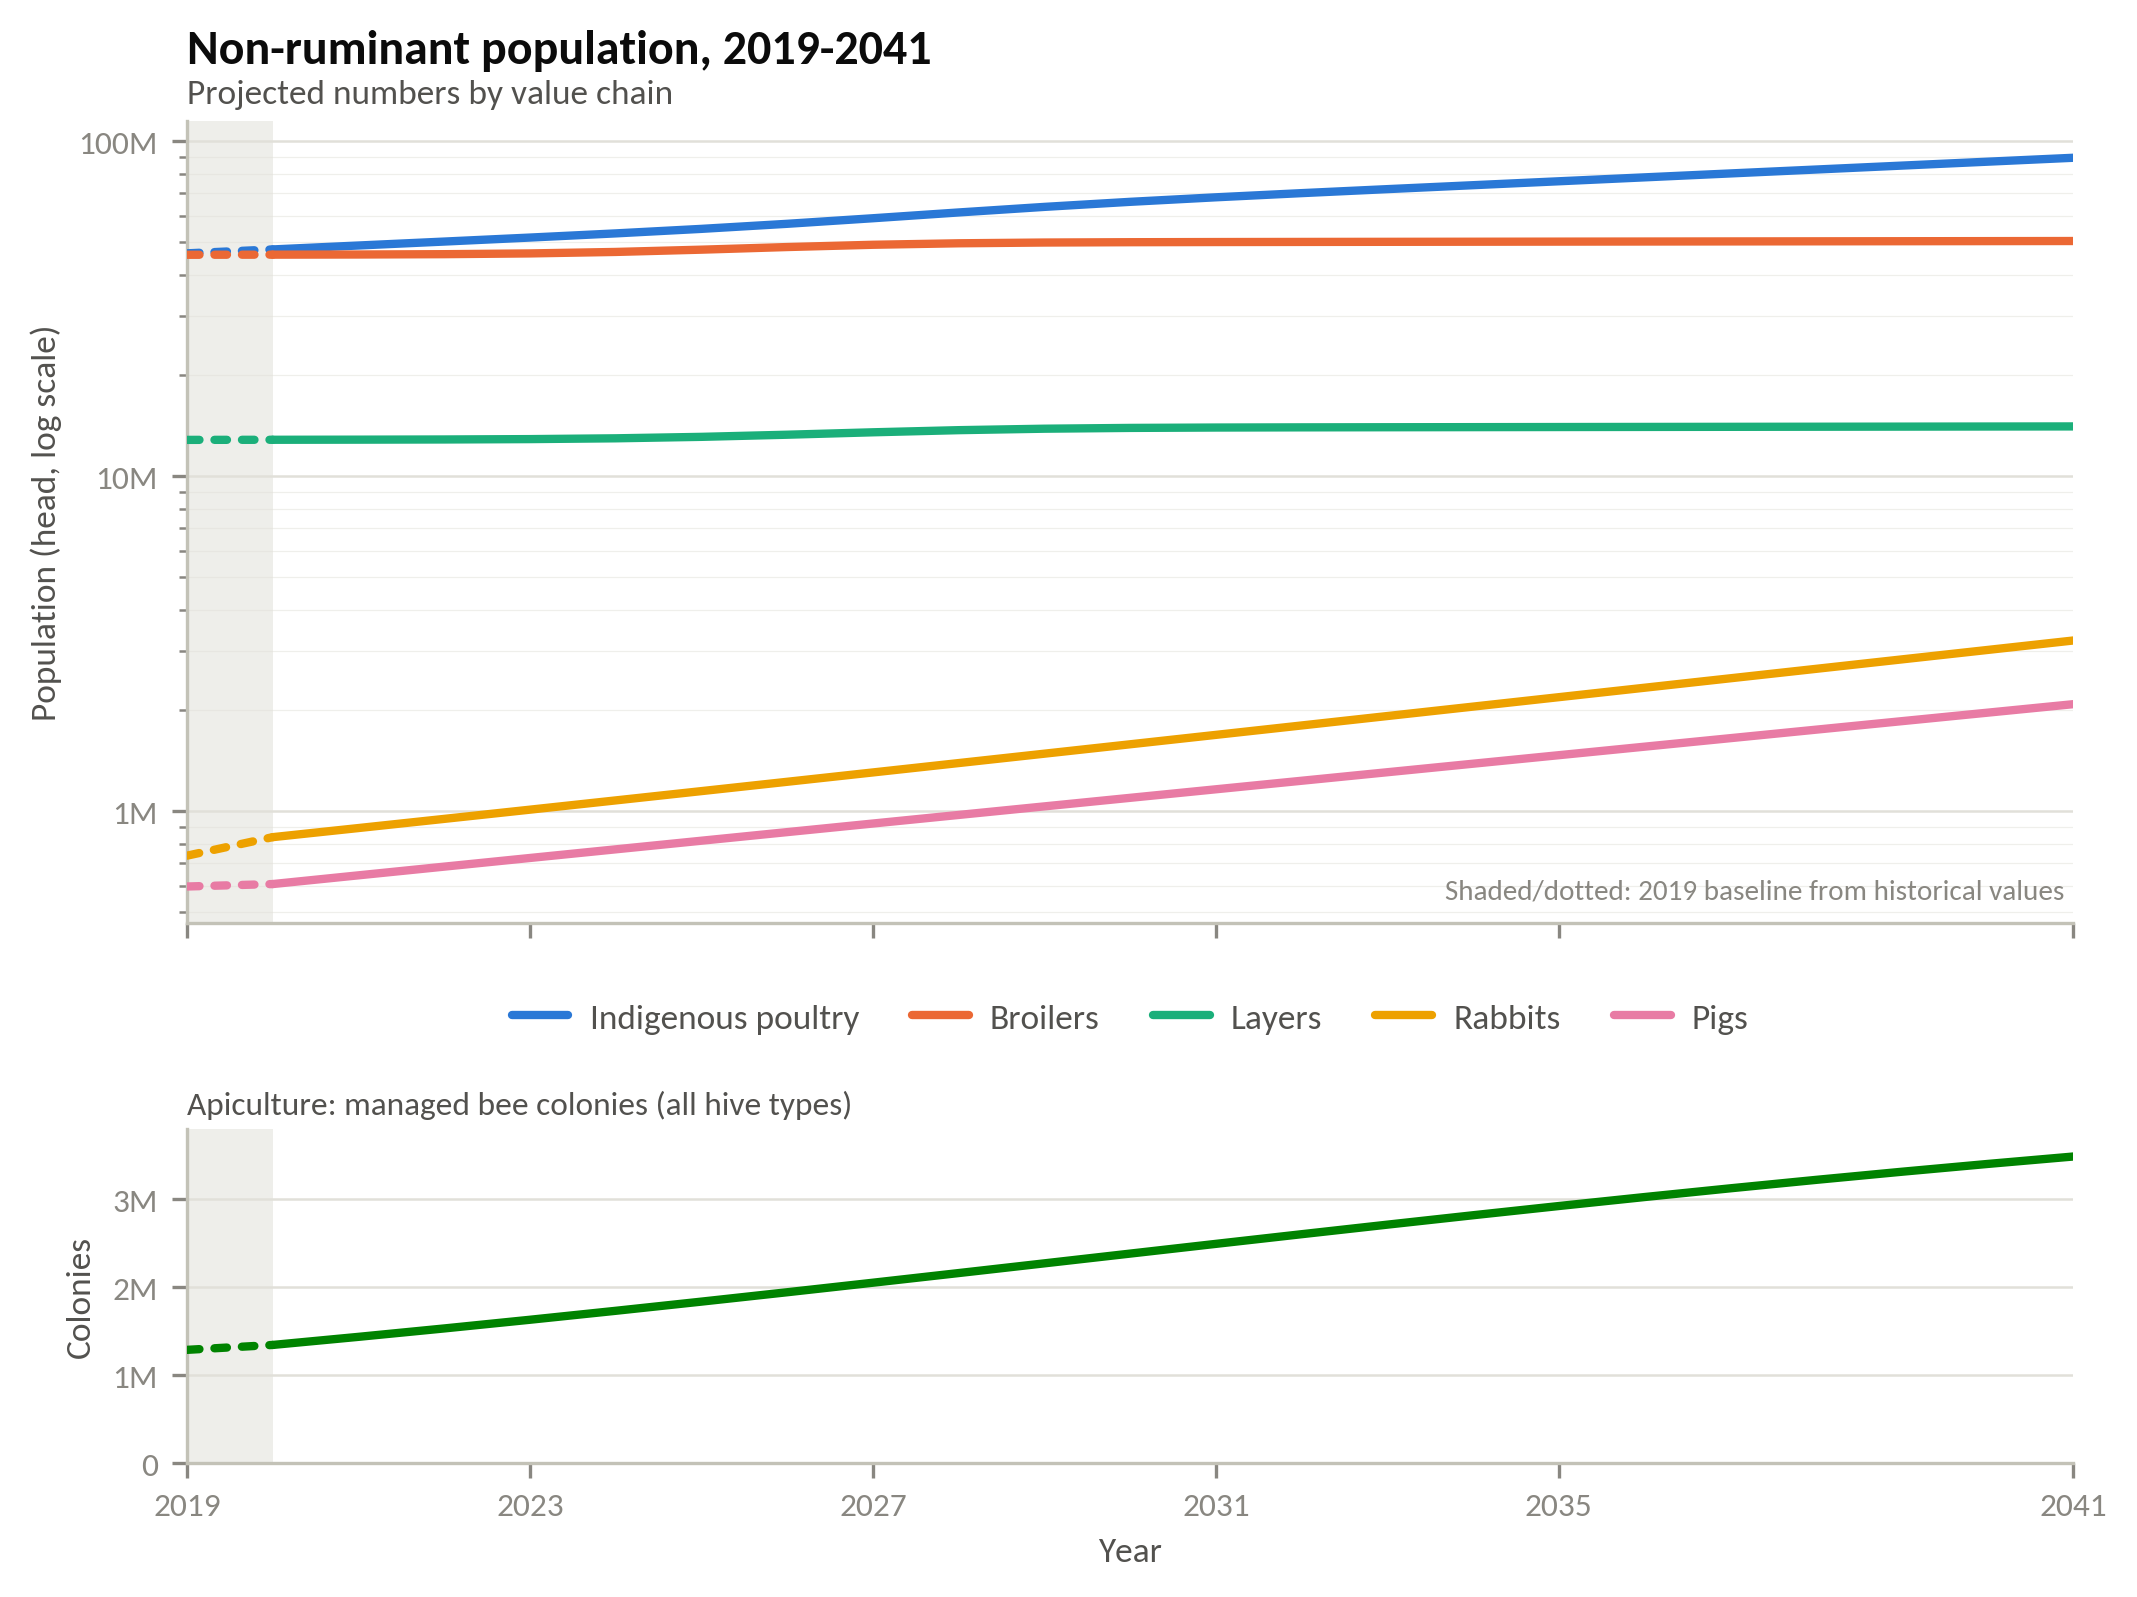
\includegraphics[width=\textwidth]{nonrum_pop.png}
\caption{Projected non-ruminant population by value chain, 2019--2041. Upper panel: livestock numbers (logarithmic axis). Lower panel: managed bee colonies (linear axis). Shaded bands and dotted segments mark the 2019 baseline, which is a historical value.}
\label{fig:nrpop}
\end{figure}

\subsection{Production}

\subsubsection{Ruminants}

Ruminant output expands across every product line (Table~\ref{tab:rumprod},
Figure~\ref{fig:rumprod}). Ten of the reported series carry a
step between the 2019 historical value and the 2020 projection
(Section~\ref{sec:dq}); for those series growth is described here from 2020, and
the 2019--2041 CAGRs in Table~\ref{tab:rumprod} should be read with that caveat.

Total milk from cattle, camels, and goats rises from 5.36 billion kg in 2020 to
15.41 billion kg in 2041, 5.2\,\% per year. Cattle milk remains the largest
single product at 9.26 billion kg in 2041; camel milk is the second largest at
5.61 billion kg, and since the two grow at almost identical rates from 2020
(5.0\,\% and 5.3\,\% per year) their ratio is close to stable, narrowing only
from 1.75:1 to 1.65:1. Goat milk is the fastest-growing dairy product at
6.6\,\% per year but remains a lot less at 531 million kg.

Meat output is led by chevon, which overtakes beef in 2020 and reaches 1.71
billion kg by 2041 against 1.37 billion kg of beef; both grow at 5.3--5.5\,\%
per year from 2020. Camel meat is the fastest-growing ruminant meat at 6.8\,\%
per year, though at 235 million kg in 2041 it remains well behind the two
leading products. Mutton grows slowest of all ruminant products at 1.2\,\% per
year from 2020, reaching 165 million kg, so the sheep chain contributes a
declining share of ruminant meat. Wool, the only product in the third group,
reaches 3.9 million kg at 2.8\,\% per year.

\begin{table}[htbp]
\centering
\caption{Ruminant production, 2019--2041 (million kg)}
\label{tab:rumprod}
\small
\begin{tabular}{lrrrrrr}
\toprule
\textbf{Series} (million kg) & \textbf{2019} & \textbf{2025} & \textbf{2030} & \textbf{2035} & \textbf{2041} & \textbf{CAGR 2019--41 (\%)} \\
\midrule
Cattle milk & 3\,087 & 4\,205 & 5\,375 & 6\,883 & 9\,263 & 5.1 \\
Camel milk & 985 & 2\,672 & 3\,369 & 4\,248 & 5\,611 & 8.2 \\
Goat milk & 156 & 222 & 292 & 383 & 531 & 5.7 \\
Chevon & 53.9 & 718 & 942 & 1\,236 & 1\,712 & 17.0 \\
Beef & 322 & 479 & 656 & 919 & 1\,375 & 6.8 \\
Camel meat & 57.6 & 104 & 139 & 178 & 235 & 6.6 \\
Mutton & 49.4 & 100 & 117 & 137 & 165 & 5.6 \\
Wool & 0.84 & 2.40 & 2.80 & 3.26 & 3.92 & 7.3 \\
\bottomrule
\end{tabular}
\end{table}

\begin{figure}[htbp]
\centering
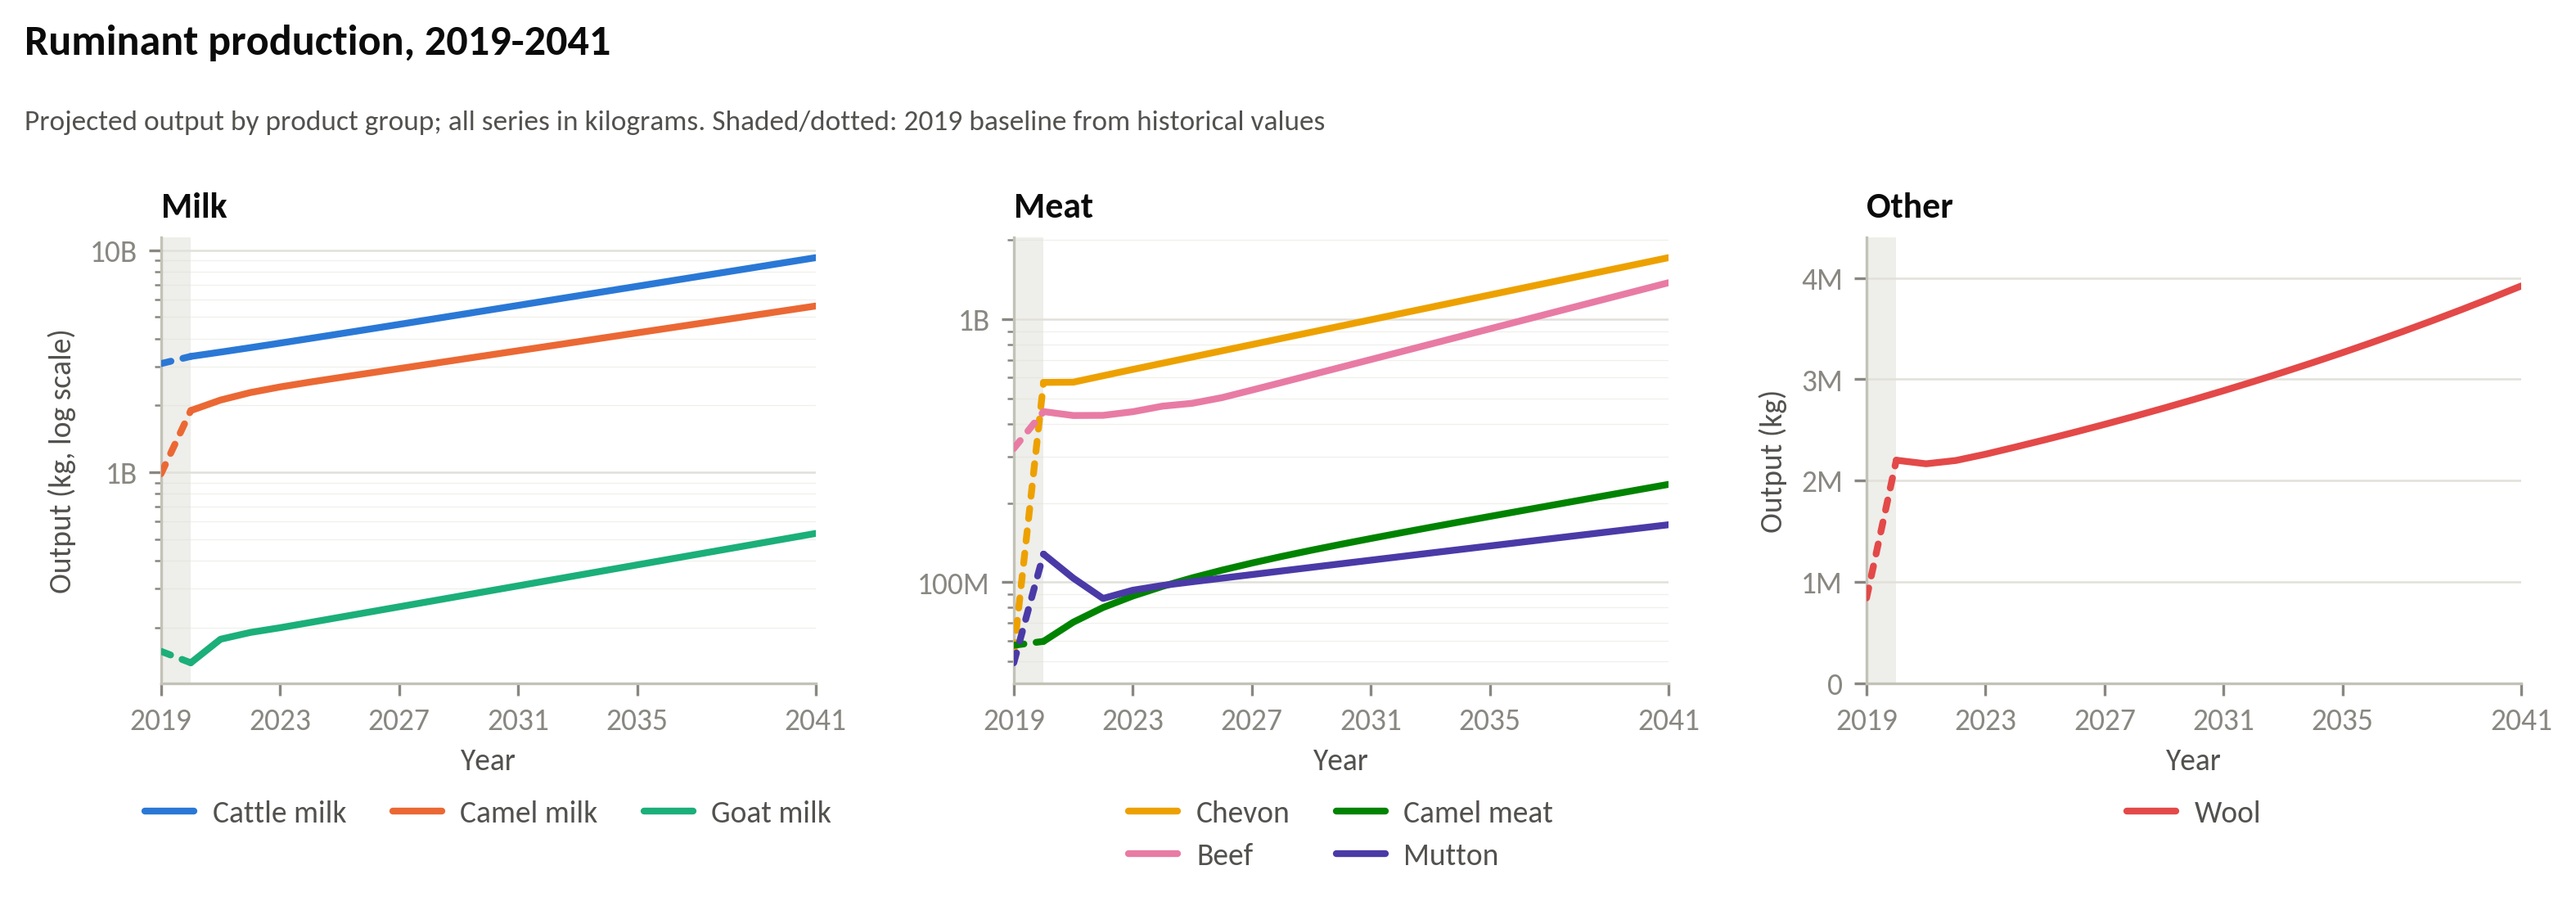
\includegraphics[width=\textwidth]{ruminant_prod.png}
\caption{Projected ruminant production, 2019--2041, by product group: milk, meat, and wool. Milk and meat panels use logarithmic vertical axes; the wool panel is linear. Shaded bands and dotted segments mark the 2019 baseline, which is a historical value.}
\label{fig:rumprod}
\end{figure}

\subsubsection{Non-ruminants}

Non-ruminant production growth is more subdued and closely tracks the population
trajectories (Table~\ref{tab:nrprod}, Figure~\ref{fig:nrprod}). Poultry meat,
the largest non-ruminant product, grows only 1.3\,\% per year to 109.7 million
kg, consistent with the plateau in commercial bird numbers. Pork grows at
4.0\,\% per year to 34.1 million kg and rabbit meat at 4.6\,\% per year (from
2020) to 4.2 million kg. The apiculture products grow fastest: honey at 5.1\,\%
per year to 41.6 million kg and beeswax at 5.4\,\% per year (from 2020) to 6.5
million kg. Honey output exceeds pork output in absolute mass from 2021 onward
and is 1.2 times pork by 2041, making apiculture the second-largest
non-ruminant product group by mass. Egg production, reported in trays and
therefore shown in its own panel on a linear axis, rises from 180.4 million
trays in 2020 to 228.7 million in 2041 (1.1\,\% per year); the 501.3 million
trays recorded for 2019 is inconsistent with the remainder of the series.

\begin{table}[htbp]
\centering
\caption{Non-ruminant production, 2019--2041 (million kg; eggs in million trays)}
\label{tab:nrprod}
\small
\begin{tabular}{lrrrrrr}
\toprule
\textbf{Series} (million) & \textbf{2019} & \textbf{2025} & \textbf{2030} & \textbf{2035} & \textbf{2041} & \textbf{CAGR 2019--41 (\%)} \\
\midrule
Poultry meat & 82.4 & 88.8 & 97.6 & 103 & 110 & 1.3 \\
Pork & 14.4 & 18.2 & 22.2 & 27.0 & 34.1 & 4.0 \\
Rabbit meat & 1.76 & 2.03 & 2.55 & 3.19 & 4.18 & 4.0 \\
Honey & 13.9 & 22.4 & 29.2 & 35.4 & 41.6 & 5.1 \\
Beeswax & 1.37 & 3.39 & 4.48 & 5.50 & 6.54 & 7.4 \\
Eggs (million trays) & 501 & 189 & 208 & 217 & 229 & -3.5 \\
\bottomrule
\end{tabular}
\end{table}

\begin{figure}[htbp]
\centering
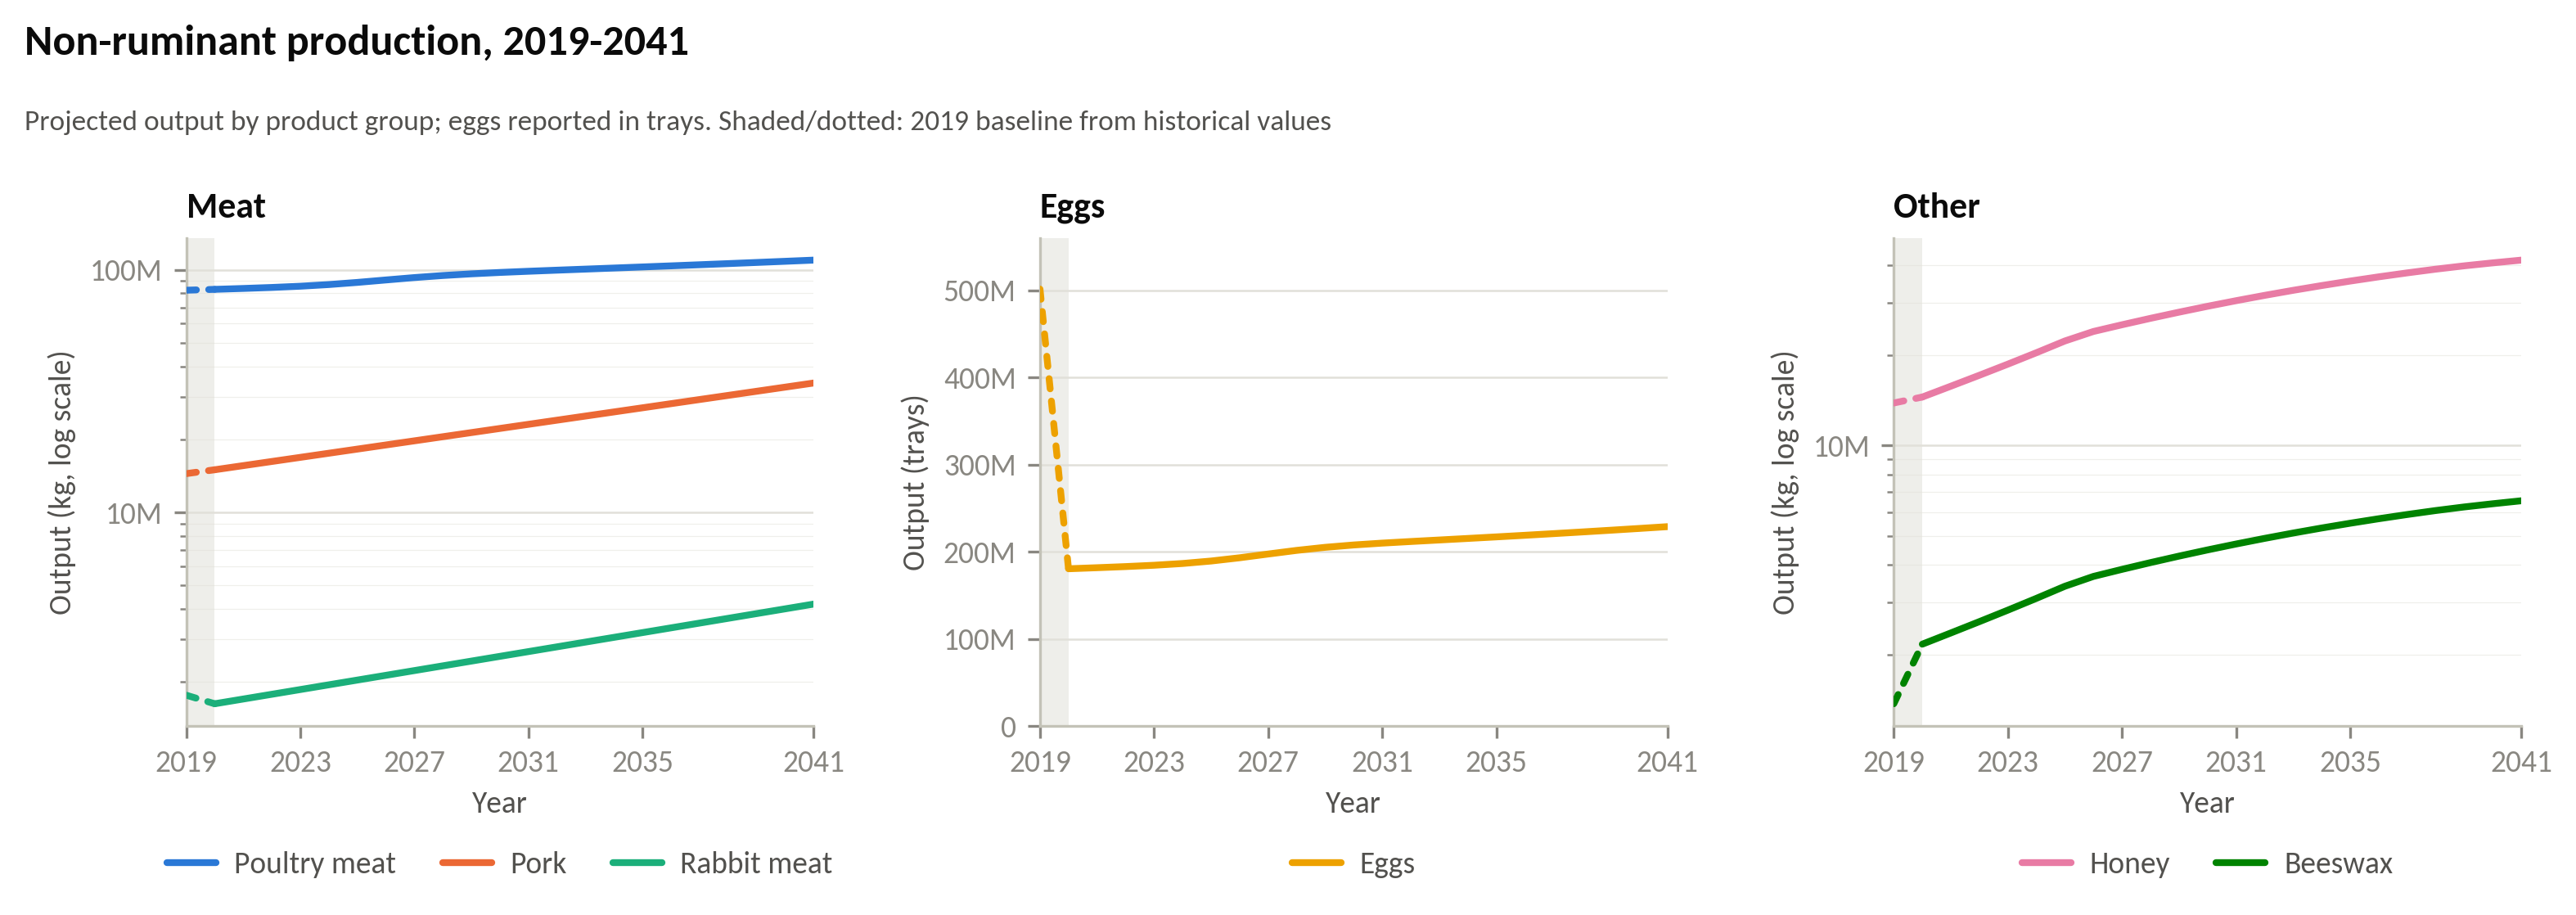
\includegraphics[width=\textwidth]{nonrum_prod.png}
\caption{Projected non-ruminant production, 2019--2041, by product group: meat, eggs, and apiculture products. Meat and other panels use logarithmic vertical axes; the egg panel is linear because eggs are reported in trays. Shaded bands and dotted segments mark the 2019 baseline, which is a historical value.}
\label{fig:nrprod}
\end{figure}

\subsection{Feed demand}

\subsubsection{Ruminants}

Ruminant chains account for the great majority of projected feed demand
(Table~\ref{tab:rumfeed}, Figure~\ref{fig:rumfeed}). Total requirement rises
from 105.8 million tonnes DM in 2020 to 353.8 million tonnes in 2041, 5.9\,\%
per year. Beef cattle alone account for 58.8 million tonnes in 2020 and 218.3
million in 2041, more than the other four ruminant chains combined in every year
of the period. Their share rises from 55.5\,\% to 61.7\,\% as they grow at
6.4\,\% per year, the fastest of the five chains. Goats follow at 6.1\,\% per
year to 36.2 million tonnes and camels at 5.6\,\% to 42.2 million tonnes, the
latter overtaking dairy cattle in 2023; dairy cattle reach 41.2 million tonnes
at 4.9\,\% per year. Sheep demand grows slowest, from 8.0 to 15.9 million
tonnes at 3.3\,\% per year.

\begin{table}[htbp]
\centering
\caption{Ruminant feed demand, 2020--2041 (thousand tonnes DM)}
\label{tab:rumfeed}
\small
\begin{tabular}{lrrrrrr}
\toprule
\textbf{Series} (\,000 t DM) & \textbf{2020} & \textbf{2025} & \textbf{2030} & \textbf{2035} & \textbf{2041} & \textbf{CAGR 2020--41 (\%)} \\
\midrule
Beef cattle & 58\,791 & 74\,615 & 104\,258 & 145\,888 & 218\,333 & 6.4 \\
Camels & 13\,474 & 19\,399 & 25\,167 & 31\,904 & 42\,184 & 5.6 \\
Dairy cattle & 15\,064 & 18\,646 & 23\,877 & 30\,584 & 41\,165 & 4.9 \\
Goats & 10\,528 & 15\,187 & 19\,929 & 26\,151 & 36\,233 & 6.1 \\
Sheep & 7\,989 & 9\,332 & 11\,135 & 13\,133 & 15\,889 & 3.3 \\
\textbf{Total ruminants} & 105\,846 & 137\,177 & 184\,366 & 247\,660 & 353\,805 & 5.9 \\
\bottomrule
\end{tabular}
\end{table}

\begin{figure}[htbp]
\centering
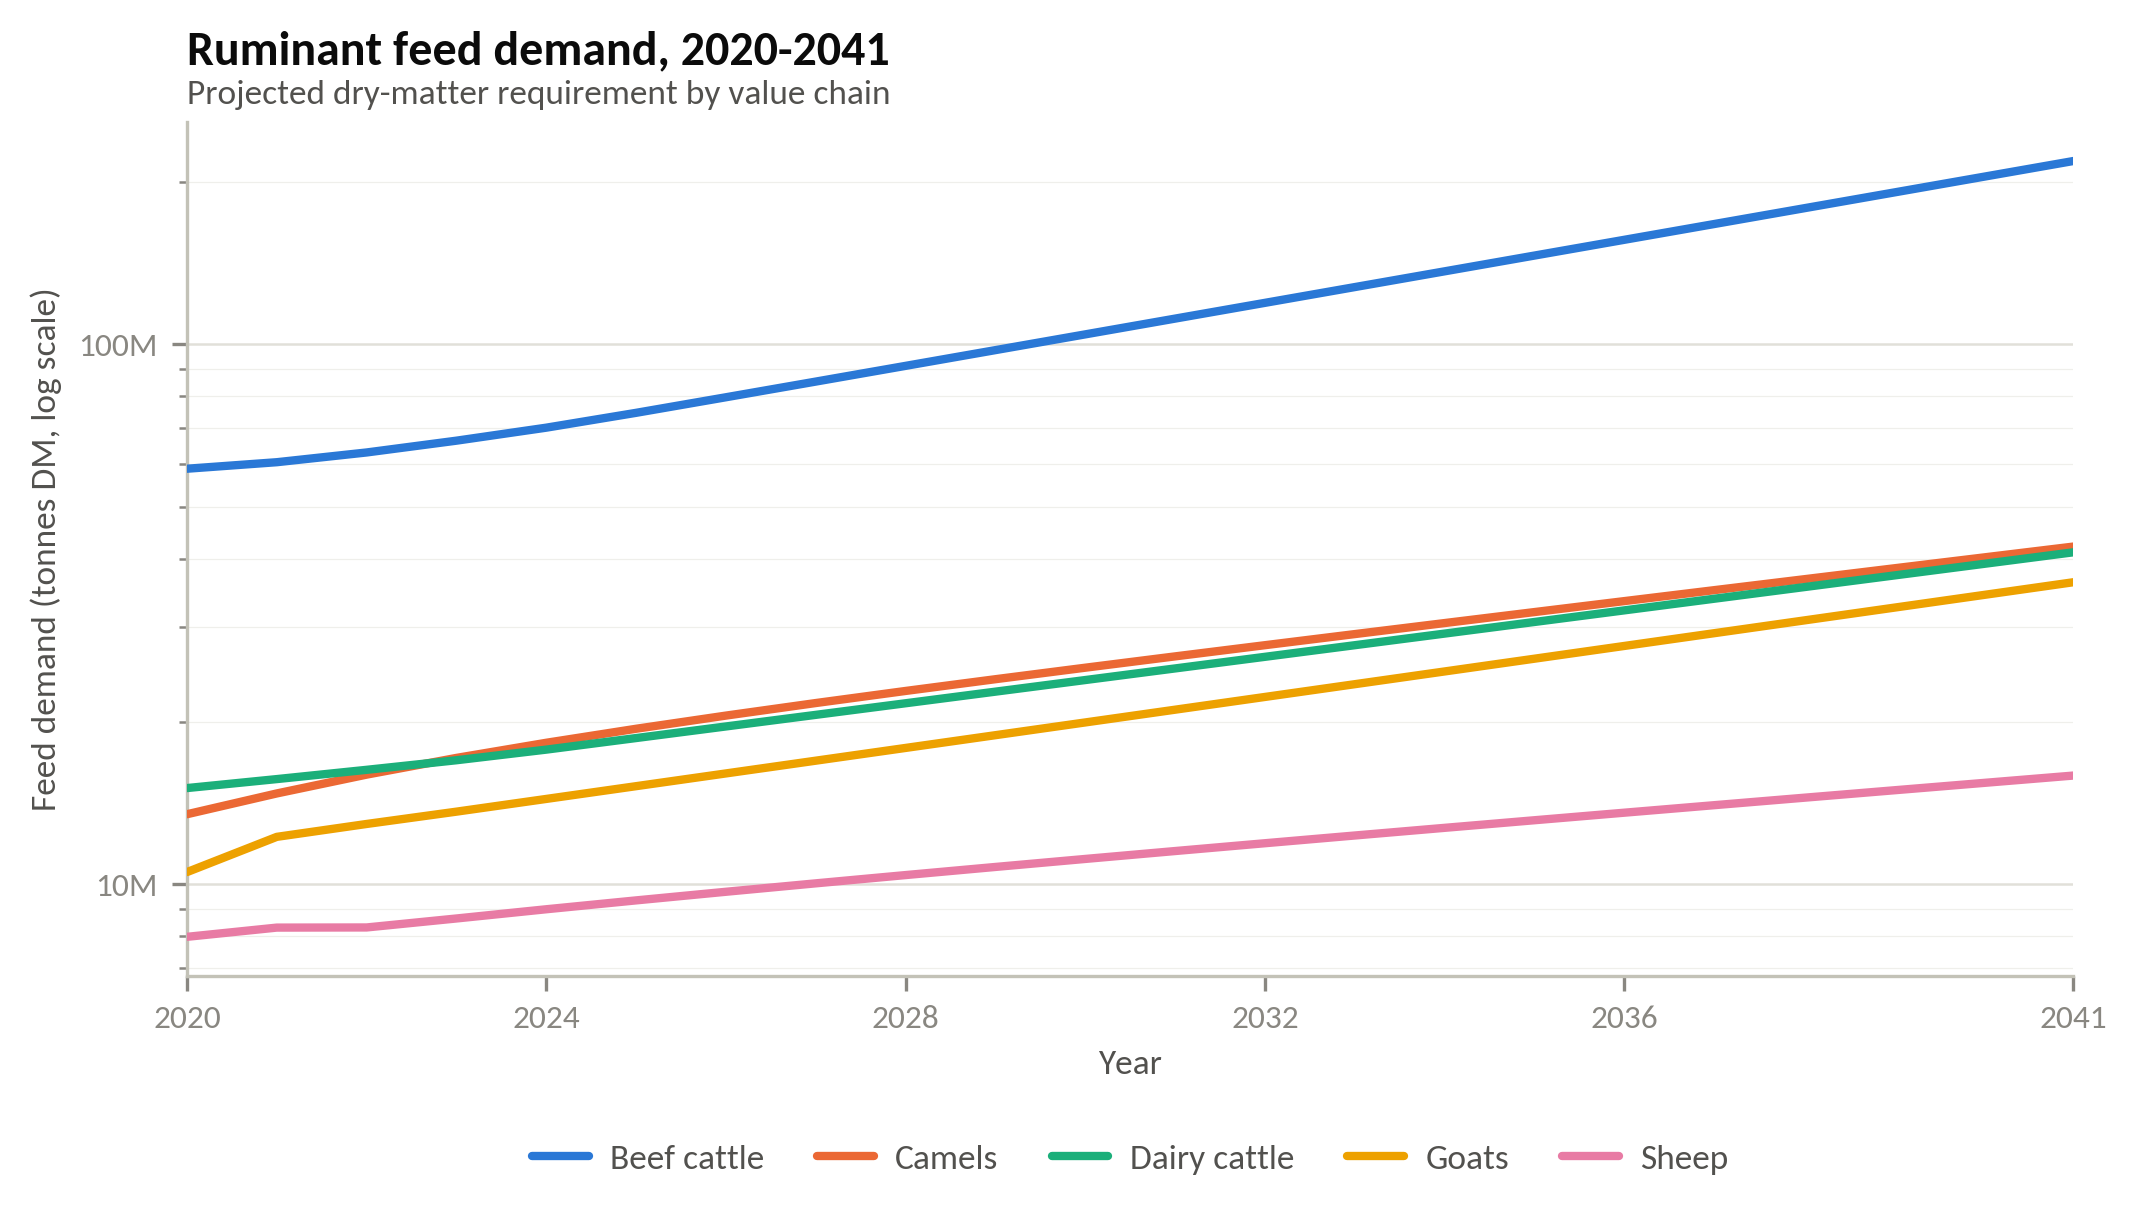
\includegraphics[width=\textwidth]{ruminant_feed.png}
\caption{Projected ruminant dry-matter feed demand by value chain, 2020--2041. Logarithmic vertical axis. (Section~\ref{sec:dq}).}
\label{fig:rumfeed}
\end{figure}

\subsubsection{Non-ruminants}

Non-ruminant feed demand is less, rising from
3.29 million tonnes in 2020 to 6.46 million tonnes in 2041 at 3.3\,\% per year
(Table~\ref{tab:nrfeed}, Figure~\ref{fig:nrfeed}). That is 1.8\,\% of the
ruminant total in 2041. Poultry accounts for the largest share throughout but grows
slowest at 1.9\,\% per year to 2.83 million tonnes, so its share falls from
57.7\,\% to 43.8\,\%. Apiculture nectar demand grows at 5.0\,\% per year to 2.49
million tonnes, reaching 88\,\% of poultry feed demand by 2041. Pig feed demand
reaches 1.09 million tonnes (4.1\,\% per year) and rabbit demand 52.7 thousand
tonnes (4.5\,\% per year).

\begin{table}[htbp]
\centering
\caption{Non-ruminant feed demand, 2020--2041 (thousand tonnes)}
\label{tab:nrfeed}
\small
\begin{tabular}{lrrrrrr}
\toprule
\textbf{Series} (\,000 t) & \textbf{2020} & \textbf{2025} & \textbf{2030} & \textbf{2035} & \textbf{2041} & \textbf{CAGR 2020--41 (\%)} \\
\midrule
Poultry & 1\,900 & 2\,067 & 2\,350 & 2\,556 & 2\,828 & 1.9 \\
Apiculture (nectar) & 900 & 1\,259 & 1\,706 & 2\,093 & 2\,489 & 5.0 \\
Pigs & 473 & 579 & 707 & 862 & 1\,092 & 4.1 \\
Rabbits & 20.9 & 25.8 & 32.2 & 40.3 & 52.7 & 4.5 \\
\textbf{Total non-ruminants} & 3\,293 & 3\,931 & 4\,795 & 5\,552 & 6\,462 & 3.3 \\
\bottomrule
\end{tabular}
\end{table}

\begin{figure}[htbp]
\centering
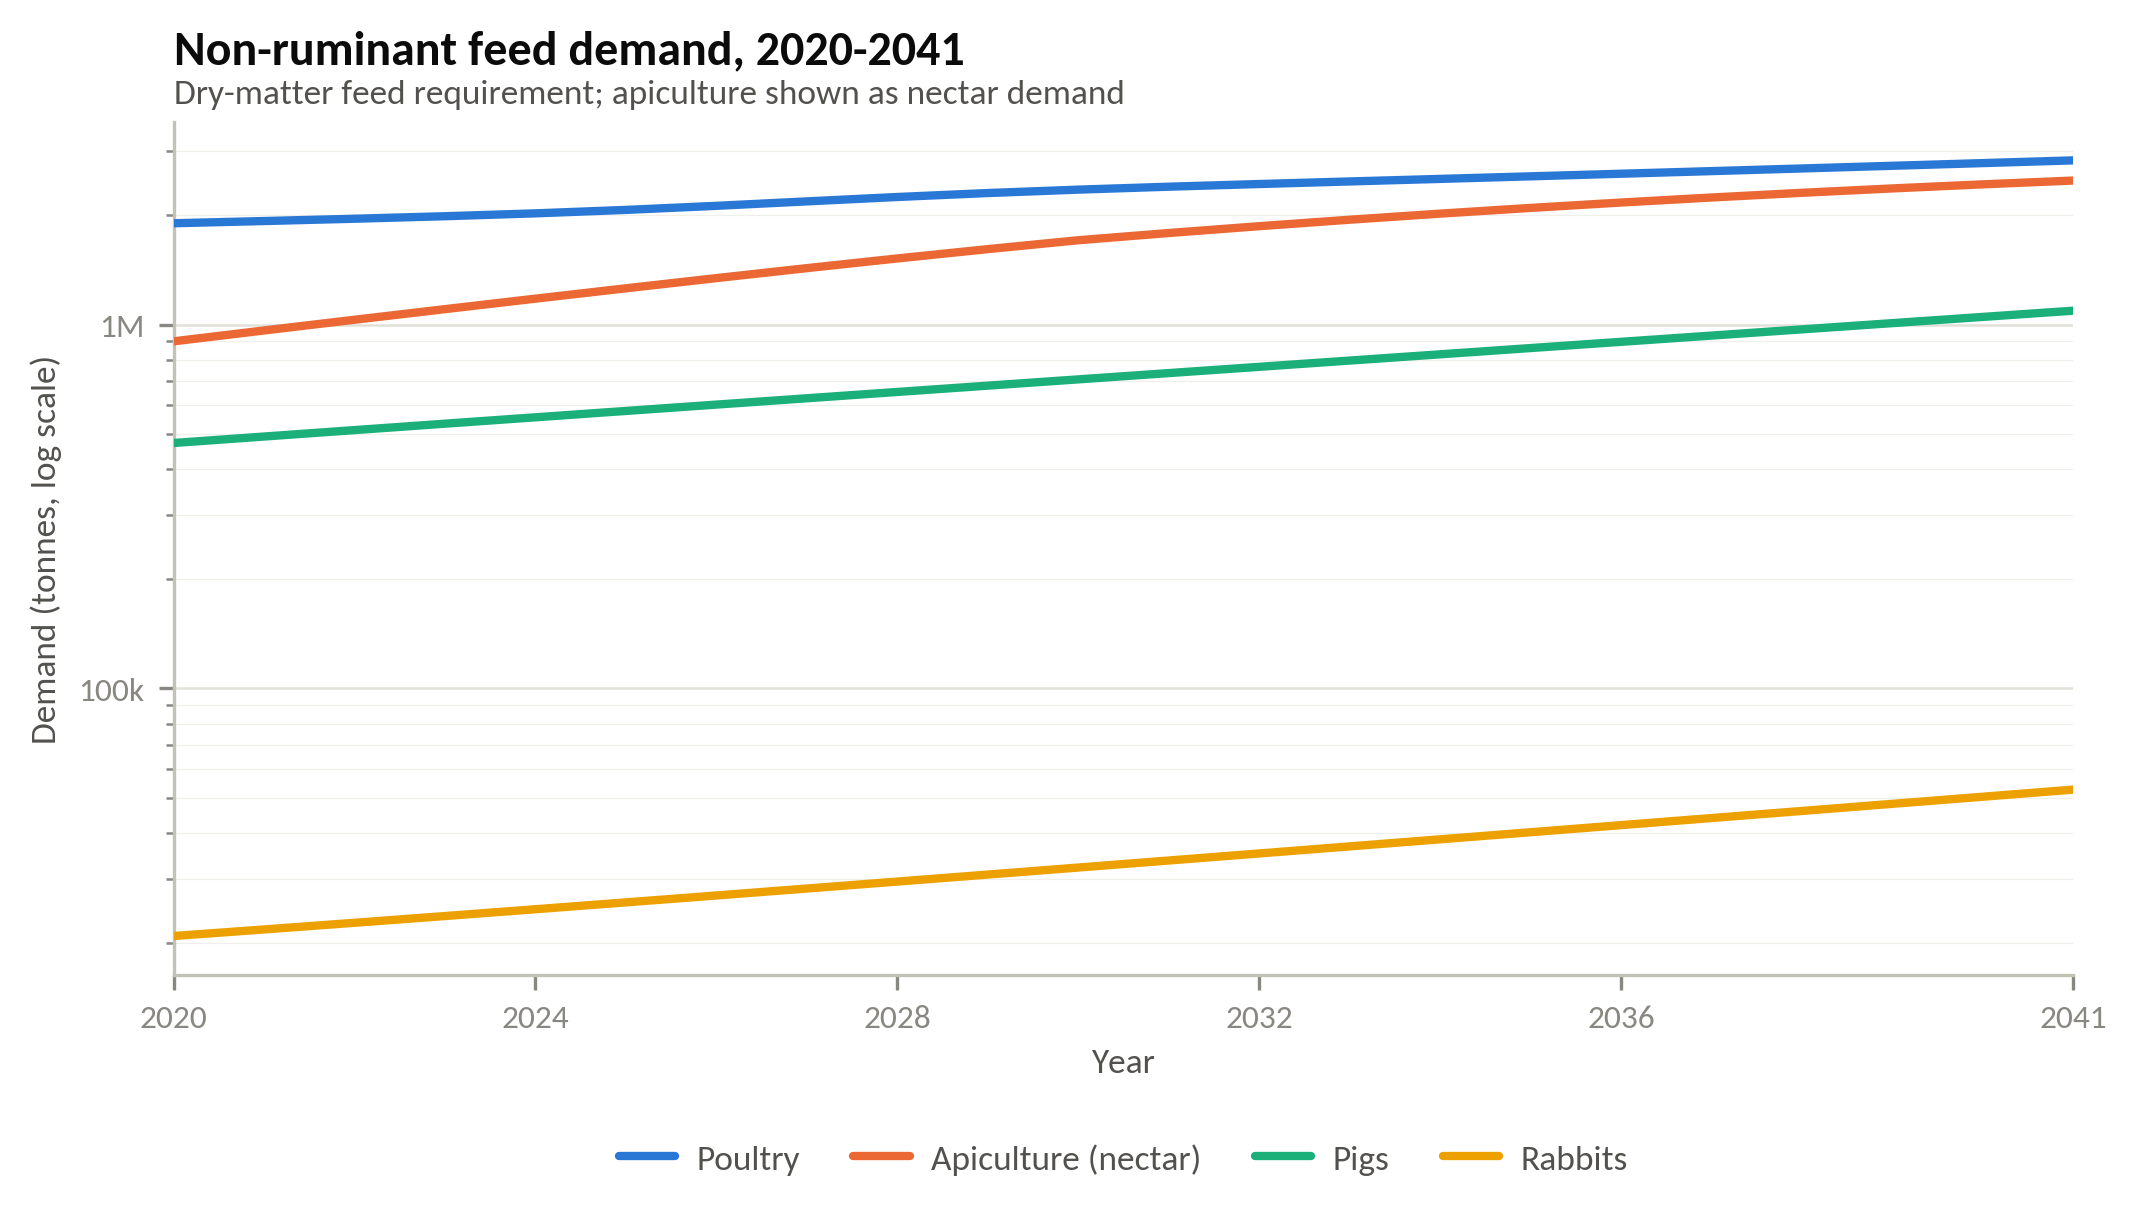
\includegraphics[width=\textwidth]{nonrum_feed.png}
\caption{Projected non-ruminant feed demand by value chain, 2020--2041. Apiculture is shown as nectar demand. Logarithmic vertical axis.}
\label{fig:nrfeed}
\end{figure}
\section{Managerial, Policy, and Societal Implications}

Beyond its forecasting function, the cohort-based framework developed in this study operates as a diagnostic instrument that translates biological herd dynamics into decision-driven intelligence. By resolving each value chain into age and sex-structured cohorts advanced on a quarterly basis, its outputs speak simultaneously to herd and enterprise managers, to national and county policymakers, and to the broader societal objectives of food security, livelihood resilience, and environmental sustainability.

\subsection{Managerial Implications}
At the enterprise level, the framework identifies precisely where within a production system growth is being lost by isolating the cohorts and transition processes that constrain performance---e.g., elevated calf, lamb, and kid mortality, depressed reproductive rates, and sub-optimal off-take structures. This granularity matters because, as seen from comparable East African rangeland systems indicates, the sale and retention rates of breeding and mature females exert the greatest influence on long-run population trajectories \cite{tuffa2017, hary2004}. 

Managers may therefore use model outputs to assess herd structure, inform culling and destocking decisions, and breeding interventions. The quarterly time step also facilitates monitoring seasonal changes in herd dynamics and feed requirements, potentially supporting early intervention where projected feed deficits or changes in herd condition indicate emerging risks \cite{meshesha2019}. 

\subsection{Policy Implications}
For national and county governments the framework directly translates into the analytical needs of national and county planning providing the value chain specific projections necessary to prioritize investment and set performance targets. The ability to run coherent forward scenarios across nine value chains provides a basis for evidence-based investment sequencing and could be institutionalized within national statistical and livestock agencies, transforming sector planning from static census snapshots to continuous data-driven foresight \cite{bosire2022}.

\subsection{Societal Implications}
At the societal scale, the framework addresses the demand-driven transformation of animal-source-food consumption that will accompany Kenya’s population growth and urbanization. Reliable projections of milk, meat, egg, and honey supply against rising demand are central to food and nutrition security planning, allowing anticipatory action on emerging supply gaps rather than reactive crisis response. Since livestock underpins the livelihoods of several million pastoralists and agro-pastoralists and constitutes the dominant source of income across the arid and semi-arid lands, the model's capacity to anticipate feed shortfalls and productivity shocks has direct implications for poverty reduction, resilience, and the protection of vulnerable rural households \cite{behnke2011}.
\section{Limitations and Opportunities for Future Research}

The model does not currently incorporate environmental carrying capacity, so projected populations are not checked against the forage, land, or water base that would ultimately constrain them. Existing carrying-capacity methods diverge substantially in both approach and result: zone-based partitioning of agro-ecological data, remote-sensing-derived stocking rates \citep{meshesha2019}, and field-sampled biomass estimates can each be applied to the same rangeland and yield different sustainable-offtake thresholds, with sensitivity analysis showing swings of up to 20 percentage points in the area classified as overutilised depending on the modelling assumptions used \citep{zandler2023}. Population models that do embed carrying capacity, such as the stochastic Boran cattle model of \citet{tuffa2017}, treat its estimation as a substantial undertaking in its own right rather than a parameter that can be added on; integrating it here, ideally partitioned by agro-ecological zone and value chain, is better scoped as an independent follow-on study.

Data availability also constrained several value chains. Camel, goat, and sheep milk are frequently reported in Kenyan statistics as a combined ``other milk'' category rather than disaggregated by species, so chain-specific dairy parameters could not always be pinned to a domestic figure. For parameters with little or no Kenyan data, values were instead drawn from studies conducted in regions with comparable climate and breeds, a substitution consistent with FAO's own finding that livestock production parameters vary widely across production systems and geographies in Sub-Saharan Africa \citep{otte2002}, and one that introduces uncertainty proportional to how closely the donor region matches Kenyan conditions.

A further limitation not covered by the data issues above is scope: because the model is first-principles and driven by biological transition rates, it does not represent exogenous shocks that can move herd trajectories independently of demography, chief among them disease outbreaks, market price swings, and policy changes. Structured population models elsewhere in the literature that couple demographic transitions to herder market decisions, such as \citet{tuffa2017}, show that offtake responses to these external drivers can materially alter population trajectories; their omission here means the projections should be read as a demographic baseline rather than a forecast robust to shocks.

Addressing these gaps points to five priorities for future work: (i) a dedicated carrying-capacity study using zone- and value-chain-specific partitioning; (ii) targeted primary data collection for the species and parameters most affected by aggregation or missing coverage; (iii) integration of economic analysis, including price and cost feedbacks; (iv) incorporation of exogenous drivers such as disease, markets, and policy, potentially via a hybrid first-principles/machine-learning extension; and (v) disaggregating each value chain into independent, and where relevant breed-specific, sub-models for finer-grained decision support.

\section{Conclusion}

This study set out to address a persistent gap in Kenya's livestock sector planning: the absence of a reproducible, data-driven framework linking herd demographics, production, and feed requirements across value chains. The resulting model resolves nine value chains, dairy cattle, beef cattle, camels, goats, sheep, poultry, pigs, rabbits, and apiculture, into age- and sex-structured cohorts advanced on a quarterly step from a 2019 baseline through 2041, translating mortality, culling, offtake, maturation, and reproduction into population, production, and feed demand trajectories for each chain.

The projections point to sustained, uneven growth across the sector. Ruminant numbers roughly triple over the horizon, led by beef cattle and goats, while non-ruminant growth is dominated by the divergence between a plateauing commercial poultry segment and a steadily expanding indigenous flock; production and feed demand follow correspondingly divergent paths by value chain. Beyond these headline trajectories, the model's cohort-level resolution surfaces the specific structural constraints, such as mortality concentrated in young cohorts, low off-take, and uneven reproductive performance, that drive them, offering a diagnostic view that aggregate, top-down projections cannot provide.

This combination of forecast and diagnosis is what gives the framework its practical value. Enterprise managers can use it to identify where herd performance is being lost and target culling, breeding, or feeding interventions accordingly; national and county planners can use it to move from static census snapshots to continuous, value-chain-specific investment and policy planning; and at the sector level, it offers a basis for anticipating feed and supply gaps before they become food security risks, particularly for the pastoralist and agro-pastoralist communities most exposed to them.

These contributions should be read alongside the limitations discussed above, chiefly the exclusion of environmental carrying capacity, gaps in Kenya-specific data for several value chains, and the omission of exogenous shocks such as disease and market fluctuations. Closing these gaps, through dedicated carrying-capacity work, targeted data collection, and extensions that incorporate economic and exogenous drivers, is the natural next step for turning this framework into a fuller decision-support tool for Kenya's livestock sector.


\backmatter

\bibliography{references}

\end{document}
